\begin{figure*}[p]
\centering

\newcommand{\codefile}[1]{%
    \lstinputlisting[
        style=mystyle,
        basicstyle=\fontsize{4.1}{4.5}\selectfont\ttfamily,
        frame=none,
        backgroundcolor=\color{white},
        aboveskip=1pt,
        belowskip=0pt,
        xleftmargin=1pt,
        xrightmargin=1pt
    ]{#1}%
}

\newcommand{\smalltitle}[1]{%
    {\fontsize{7}{7.5}\selectfont\bfseries #1}
}

\begin{tcolorbox}[
    width=\textwidth,
    colback=magenta!3,
    colframe=purple!40,
    title=Example with TikZ Code,
    enhanced,
    sharp corners=south,
    boxrule=0.5pt,
    left=2mm,
    right=2mm,
    top=1mm,
    bottom=1mm
]

\begin{minipage}[t]{0.29\linewidth}
\centering
\smalltitle{Source}

\vspace{1mm}

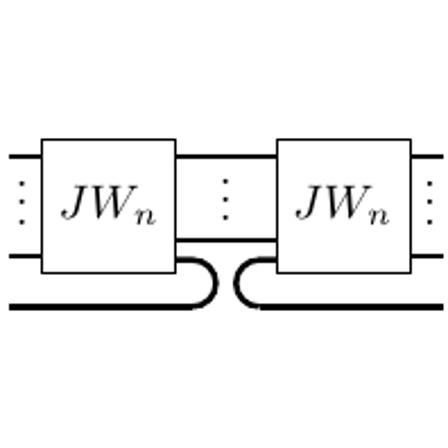
\includegraphics[
    width=\linewidth,
    height=2.9cm,
    keepaspectratio
]{structure/examples_new/sample_0549_source.png}
\end{minipage}
%
\hfill
%
\begin{minipage}[t]{0.36\linewidth}
\centering
\smalltitle{Edit Instruction}

\vspace{-2mm}

\begin{tcolorbox}[
    colback=white,
    colframe=gray!45,
    boxrule=0.3pt,
    arc=1mm,
    left=1mm,right=1mm,
    top=1mm,bottom=1mm
]
\raggedright
\fontsize{5.4}{6.1}\selectfont
    Remove the right-hand $JW_n$ box, its external input/output lines, and the far-right vertical ellipsis. Remove the two horizontal lines. Move the loop from the gap between the boxes to a position beneath the remaining box, where it connects around the lower-left and lower-right sides. Increase the height of the remaining box upward from 2.0 to 2.3 units; the loop remains below the box rather than being contained within its vertical span. Reposition the two left input lines and the left and right vertical ellipses to suit the taller single-box layout.
\end{tcolorbox}
\end{minipage}
%
\hfill
%
\begin{minipage}[t]{0.29\linewidth}
\centering
\smalltitle{Ground Truth}

\vspace{1mm}

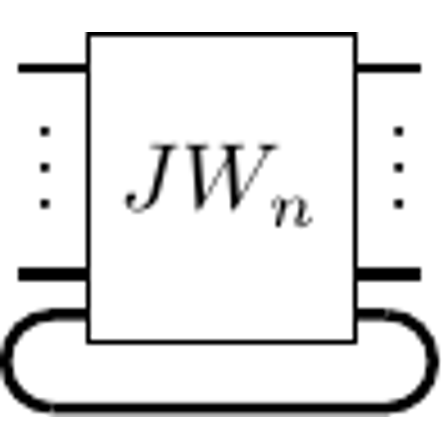
\includegraphics[
    width=\linewidth,
    height=2.9cm,
    keepaspectratio
]{structure/examples_new/sample_0549_gt.png}
\end{minipage}

\vspace{2mm}

\begin{minipage}[t]{0.44\linewidth}
\vspace{0pt}
\begin{tcolorbox}[
    width=\linewidth,
    colback=white,
    colframe=gray!45,
    boxrule=0.3pt,
    arc=1mm,
    left=0.5mm,right=0.5mm,
    top=0.5mm,bottom=0.5mm
]
\codefile{structure/examples_new/sample_0549_source.tex}
\end{tcolorbox}
\end{minipage}
%
\hfill
%
\begin{minipage}[t]{0.44\linewidth}
\vspace{0pt}
\begin{tcolorbox}[
    width=\linewidth,
    colback=white,
    colframe=gray!45,
    boxrule=0.3pt,
    arc=1mm,
    left=0.5mm,right=0.5mm,
    top=0.5mm,bottom=0.5mm
]
\codefile{structure/examples_new/sample_0549_gt.tex}
\end{tcolorbox}
\end{minipage}

\vspace{1mm}

\tcblower

\begin{minipage}[t]{0.485\linewidth}
\centering
\smalltitle{Gemini-3.1-Pro}

\vspace{1mm}

\begin{tikzpicture}
\node[inner sep=0] (img) {%
    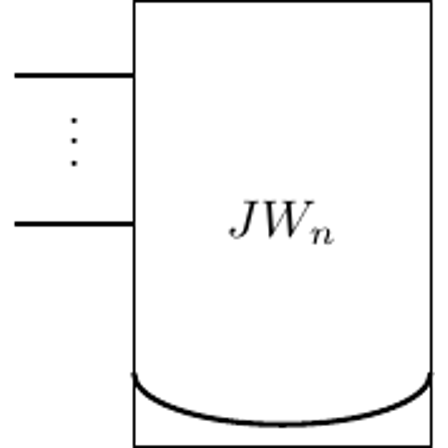
\includegraphics[
        width=0.72\linewidth,
        height=2.9cm,
        keepaspectratio
    ]{structure/examples_new/sample_0549_gemini.png}%
};

\node[
    anchor=west,
    right=1.5mm of img.east,
    align=left,
    fill=white,
    draw=gray!45,
    line width=0.3pt,
    rounded corners=1mm,
    inner xsep=1mm,
    inner ysep=0.8mm
] {%
    \fontsize{5.0}{5.8}\selectfont
    \begin{tabular}{@{}lr@{}}
    \textbf{TED}  & 0.680 \\
    \textbf{DSim} & 0.758 \\
    \textbf{EA}   & 0.500 \\
    \textbf{SP}   & 0.600 \\
    \textbf{VQ}   & 0.700 \\
    \textbf{AT}   & 165
    \end{tabular}
};
\end{tikzpicture}

\vspace{1mm}

\begin{tcolorbox}[
    colback=white,
    colframe=gray!45,
    boxrule=0.3pt,
    arc=1mm,
    left=0.5mm,right=0.5mm,
    top=0.5mm,bottom=0.5mm
]
\codefile{structure/examples_new/sample_0549_gemini.tex}
\end{tcolorbox}
\end{minipage}
%
\hfill
%
\begin{minipage}[t]{0.485\linewidth}
\centering
\smalltitle{EdiTikZ-9B-RL}

\vspace{1mm}

\begin{tikzpicture}
\node[inner sep=0] (img) {%
    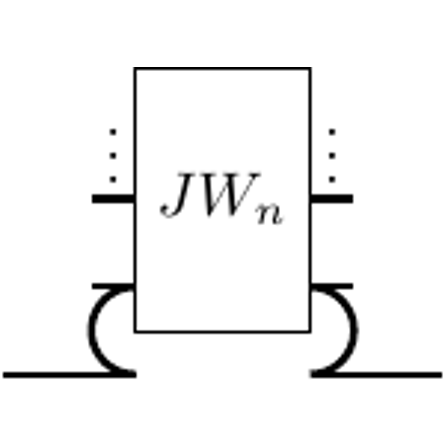
\includegraphics[
        width=\linewidth,
        height=2.9cm,
        keepaspectratio
    ]{structure/examples_new/sample_0549_9b_rl.png}%
};

\node[
    anchor=west,
    right=1.5mm of img.east,
    align=left,
    fill=white,
    draw=gray!45,
    line width=0.3pt,
    rounded corners=1mm,
    inner xsep=1mm,
    inner ysep=0.8mm
] {%
    \fontsize{5.0}{5.8}\selectfont
    \begin{tabular}{@{}lr@{}}
    \textbf{TED}  & 0.659 \\
    \textbf{DSim} & 0.898 \\
    \textbf{EA}   & 0.500 \\
    \textbf{SP}   & 0.900 \\
    \textbf{VQ}   & 0.800 \\
    \textbf{AT}   & 323
    \end{tabular}
};
\end{tikzpicture}

\vspace{1mm}

\begin{tcolorbox}[
    colback=white,
    colframe=gray!45,
    boxrule=0.3pt,
    arc=1mm,
    left=0.5mm,right=0.5mm,
    top=0.5mm,bottom=0.5mm
]
\codefile{structure/examples_new/sample_0549_9b_rl.tex}
\end{tcolorbox}
\end{minipage}

\end{tcolorbox}

\caption{TikZ programs and rendered figures for a representative scientific-figure edit. Models receive the source figure and edit instruction and generate the edited TikZ program. Per-example TED, DSim, EA, SP, VQ, and AT are shown beside each prediction.}
\label{fig:tikz_code_example_2}

\end{figure*}